%%%%%%%%%%%%%%%%%%%%%%%%%%%%%%%%%%%%%%%%%%%%%%%%%%%%%%%%%%%%%%%%%%%%%%%%%%%%%%%%%%%
%% This project aims to create the template for presentation.                   %%
%% author: Luigi Durso                                                          %%
%% contacts:                                                                    %%
%%    e-mail: luigi.durso@si2001.it                                             %%
%%    linktree: https://linktr.ee/maumneto                                      %%
%%%%%%%%%%%%%%%%%%%%%%%%%%%%%%%%%%%%%%%%%%%%%%%%%%%%%%%%%%%%%%%%%%%%%%%%%%%%%%%%%%%
\documentclass{../libs/presentation_format}
% Inserting the preamble file with the packages
%%%%%%%%%%%%%%%%%%%%%%%%%%%%%%%%%%%%%%%%%%%%%%%%%%%%%%%%%%%%%%%%%%%%%
%% This file contains the packages that can be used in the beamer. %%
%%%%%%%%%%%%%%%%%%%%%%%%%%%%%%%%%%%%%%%%%%%%%%%%%%%%%%%%%%%%%%%%%%%%%
% Package to fonts family
\usepackage[T1]{fontenc}
% Package to accentuation
\usepackage[utf8]{inputenc}
% Package to Italian language
\usepackage[italian]{babel}
% Package to Figures
\usepackage{graphicx}
\usepackage{caption}
\usepackage{subcaption}
% Package to the colors
\usepackage{color}
% Package to the colors
\usepackage{xcolor}
% Packages to math symbols and expressions
\usepackage{amsfonts, amssymb, amsmath}
% Package to multiple lines and columns in table
\usepackage{multirow, array} 
% Package to create pseudo-code
% For more detail of this package: http://linorg.usp.br/CTAN/macros/latex/contrib/algorithm2e/doc/algorithm2e.pdf
\usepackage{algorithm2e}
% Package to insert code
\usepackage{listings} 
\usepackage{keyval}
% Package to justify text
\usepackage[document]{ragged2e}
% Package to manage the bibliography
\usepackage[backend=biber, style=numeric, sorting=none]{biblatex}
% Package to facilities quotations
\usepackage{csquotes}
% Package to use multicols
\usepackage{multicol}
% Inserting the references file
\bibliography{../references.bib}

% Title
\title[Flutter-Dart]{\huge\textbf{Flutter e Dart - Le basi}}
% Subtitle
\subtitle{Flutter - Gestione dello stato}
% Author of the presentation
\author{Luigi Durso}
% Company's Name
\institute[SI2001]{
    % email for contact
    \normalsize{\email{luigi.durso@si2001.it}}
    \newline
    \centering
    
\includegraphics[scale=0.3]{../libs/emblem.png}
    \newline
    % company name
    \company
}
% date of the presentation
\date{\today}


%%%%%%%%%%%%%%%%%%%%%%%%%%%%%%%%%%%%%%%%%%%%%%%%%%%%%%%%%%%%%%%%%%%%%%%%%%%%%%%%%%
%% Start Document of the Presentation                                           %%               
%%%%%%%%%%%%%%%%%%%%%%%%%%%%%%%%%%%%%%%%%%%%%%%%%%%%%%%%%%%%%%%%%%%%%%%%%%%%%%%%%%
\begin{document}
% insert the code style
%%%%%%%%%%%%%%%%%%%%%%%%%%%%%%%%%%%%%%%%%%%%%%%%%%%%%%%%%%%%%%%%%%%%%%%%%%%%%%%%%%%
%% This file contains the style of the codes show in slides.                     %%
%% The package used is listings, but it possible to used others.                 %%
%%%%%%%%%%%%%%%%%%%%%%%%%%%%%%%%%%%%%%%%%%%%%%%%%%%%%%%%%%%%%%%%%%%%%%%%%%%%%%%%%%%

% color used in the code style
\definecolor{codegreen}{rgb}{0,0.6,0}
\definecolor{codegray}{rgb}{0.5,0.5,0.5}
\definecolor{codepurple}{rgb}{0.58,0,0.82}
\definecolor{codebackground}{rgb}{0.95,0.95,0.92}

% style of the code!
\lstdefinestyle{codestyle}{
    backgroundcolor=\color{codebackground},   
    commentstyle=\color{codegreen},
    keywordstyle=\color{magenta},
    numberstyle=\tiny\color{codegray},
    stringstyle=\color{codepurple},
    basicstyle=\ttfamily\footnotesize,
    frame=single,
    breakatwhitespace=false,         
    breaklines=true,                 
    captionpos=b,                    
    keepspaces=true,                 
    numbers=left,                    
    numbersep=5pt,                  
    showspaces=false,                
    showstringspaces=false,
    showtabs=false,                  
    tabsize=2,
    title=\lstname 
}

\lstset{style=codestyle}

\lstset{basicstyle=\ttfamily,
	showstringspaces=false,
	commentstyle=\color{red},
	keywordstyle=\color{blue},
	inputencoding=utf8,
	extendedchars=true
}


%% ---------------------------------------------------------------------------
% First frame (with tile, subtitle, ...)
\begin{frame}{}
    \maketitle
\end{frame}

%% ---------------------------------------------------------------------------
% Table of content frame
\begin{frame}{Sommario}
    \begin{multicols}{2}
        \tableofcontents
    \end{multicols}
\end{frame}

%% ---------------------------------------------------------------------------

\section{Lezione precedente}
\begin{frame}{Un po' di codice}
\begin{tabular}{lll}
	\raisebox{-.5\height}{
\includegraphics[scale=0.3]{../libs/Developer-Friendly.png}}
	\emph{Analizziamo l'elaborato precedente!}\\
\end{tabular}
\end{frame}

%% ---------------------------------------------------------------------------

\section{Problema}
\begin{frame}{Stato condiviso}
	\begin{minipage}[0.2\textheight]{\textwidth}
		\begin{columns}[T]
			\begin{column}{0.4\textwidth}
				\begin{figure}[htpb]
					\centering
					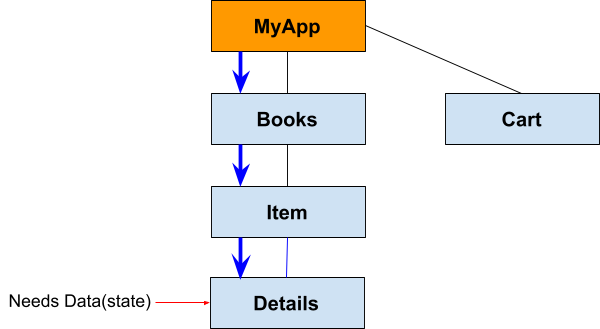
\includegraphics[scale=0.2]{../libs/state-management-problem}
				\end{figure}
			\end{column}
			\begin{column}{0.6\textwidth}
				\emph{Qual'è il problema?}
				\begin{itemize}
					\item Dati condivisi tra più livelli dell'albero dei widgets
					\item Richiesta di passaggio di parametri anche in widget che non ne hanno bisogno
					\item Re-build eseguita su tutto il percorso di dipendenze
				\end{itemize}
			\end{column}
		\end{columns}
	\end{minipage}
\end{frame}

%% ---------------------------------------------------------------------------

\begin{frame}{Idee di soluzione}
	\emph{Un possibile approccio di soluzione}
	\begin{itemize}
		\item Pensare allo stato disaccoppiato dai widgets
		\item Interazione tra widget e stato attraverso eventi e funzioni
		\item Ogni widget si sottoscrive ai cambiamenti della parte di stato a cui è interessato
	\end{itemize}
\end{frame}

%% ---------------------------------------------------------------------------

\begin{frame}{Soluzioni}
	\begin{figure}[htpb]
		\centering
		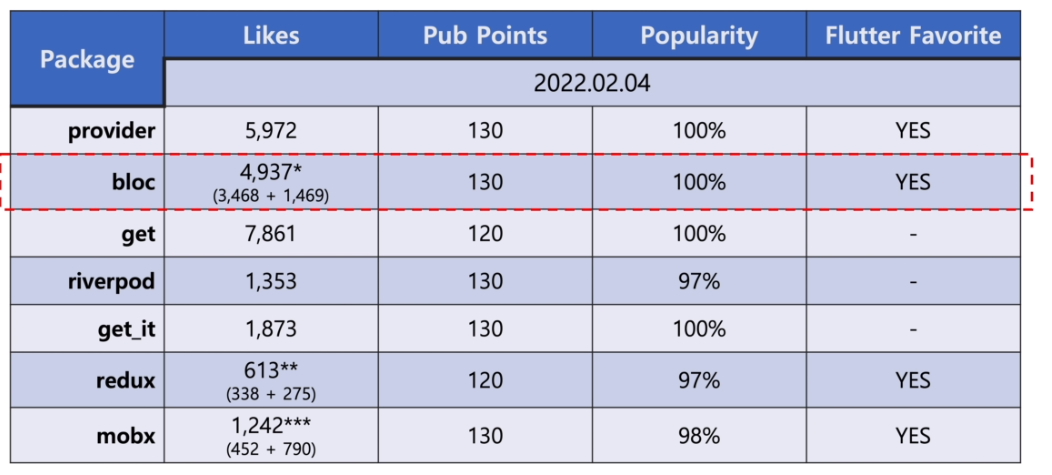
\includegraphics[width=9cm]{../libs/state-management-stats}
	\end{figure}
\end{frame}

%% ---------------------------------------------------------------------------

\section{BLoC - Cosa}
\begin{frame}{BLoC}
	\begin{figure}[htpb]
		\centering
		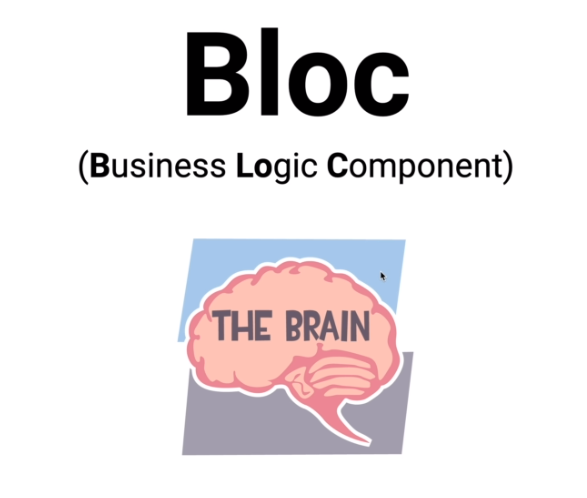
\includegraphics[width=9cm]{../libs/bloc-first-logo}
	\end{figure}
\end{frame}

%% ---------------------------------------------------------------------------

\begin{frame}{Perché usare BLoC}
	\emph{Bloc segue tre principi fondamentali:}
	\begin{itemize}
		\item \emph{Semplicità}: Facile da imparare, chiunque può approcciarsi facilmente a questa tecnologia.
		\item \emph{Potenza}: Attraverso la creazione di piccoli componenti si può creare un'applicativo di grande complessità.
		\item \emph{Testabilità}: Ogni aspetto dell'applicativo è facilmente testabile.
	\end{itemize}
\end{frame}

%% ---------------------------------------------------------------------------

\begin{frame}{Approcci diversi}
	\emph{Possiamo usare approcci diversi in base alle nostre esigenze:}
	\begin{itemize}
		\item Approccio event-driven con \emph{BLoC}
		\item Approccio basato su funzioni con \emph{Cubit}
	\end{itemize}
\end{frame}

%% ---------------------------------------------------------------------------

\begin{frame}{Struttura di BLoC}
	\begin{minipage}[0.2\textheight]{\textwidth}
		\begin{columns}[T]
			\begin{column}{0.4\textwidth}
				\begin{figure}[htpb]
					\centering
					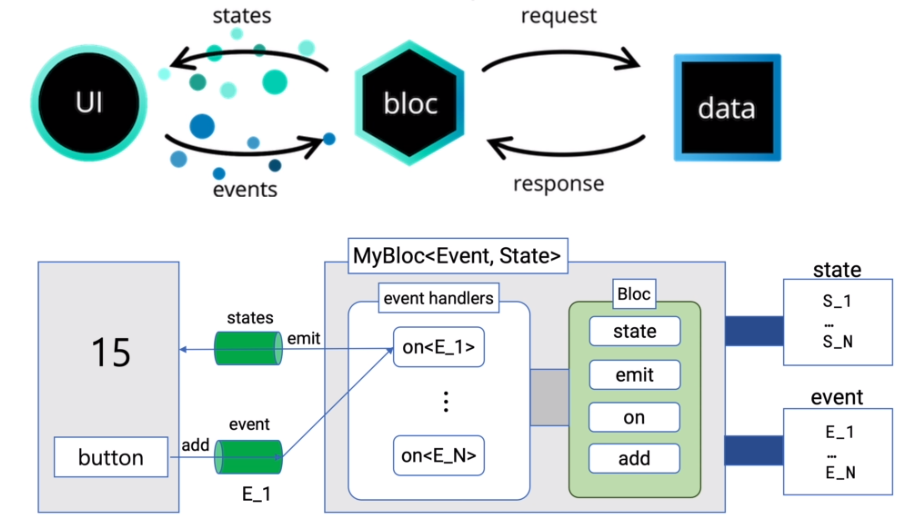
\includegraphics[scale=0.15]{../libs/bloc-structure}
				\end{figure}
			\end{column}
			\begin{column}{0.6\textwidth}
				\begin{itemize}
					\item Lettura degli eventi scatenati dalla UI
					\item Ricezione dell'evento e gestione mediante il giusto event handler
					\item Elaborazione dell'evento ( Es. Interazione con Repository )
					\item Rendering del nuovo stato nella UI
				\end{itemize}
			\end{column}
		\end{columns}
	\end{minipage}
\end{frame}

%% ---------------------------------------------------------------------------

\begin{frame}{Cosa possiamo osservare}
	\begin{figure}[htpb]
		\centering
		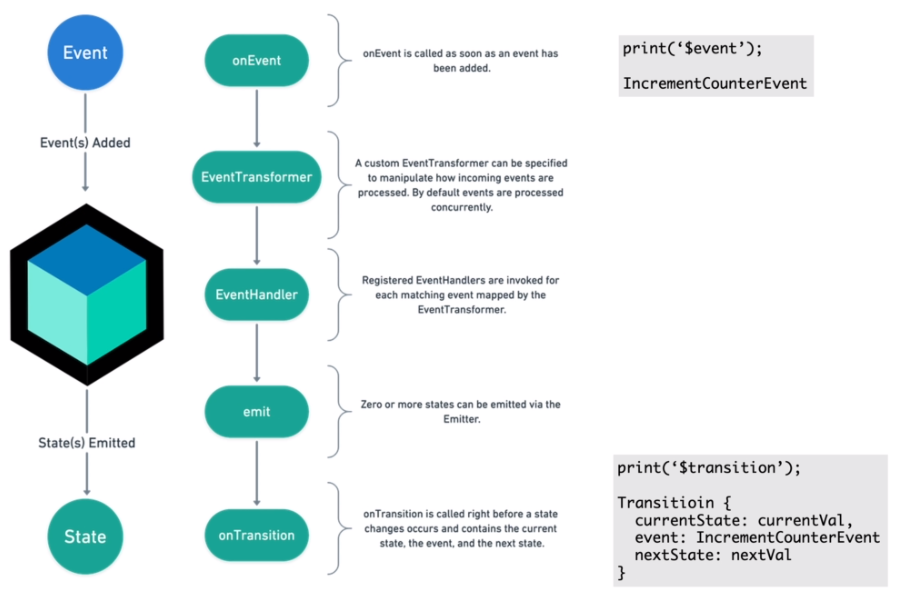
\includegraphics[width=9cm]{../libs/bloc-flow}
	\end{figure}
\end{frame}

%% ---------------------------------------------------------------------------

\begin{frame}{Event transformation}
	\begin{figure}[htpb]
		\centering
		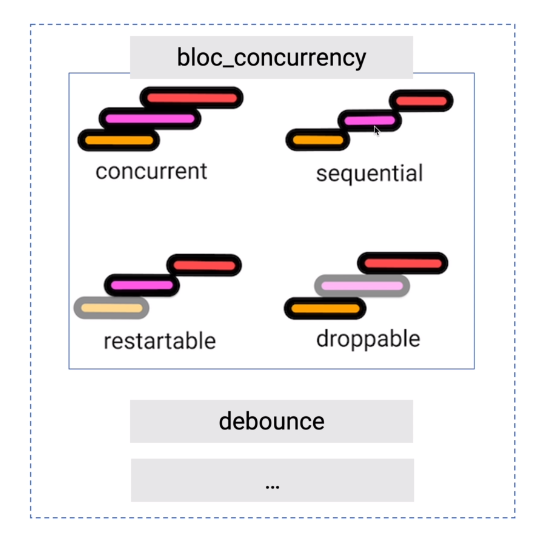
\includegraphics[width=5cm]{../libs/event-transformation}
	\end{figure}
\end{frame}

%% ---------------------------------------------------------------------------

\begin{frame}{Struttura di Cubit}
	\begin{figure}[htpb]
		\centering
		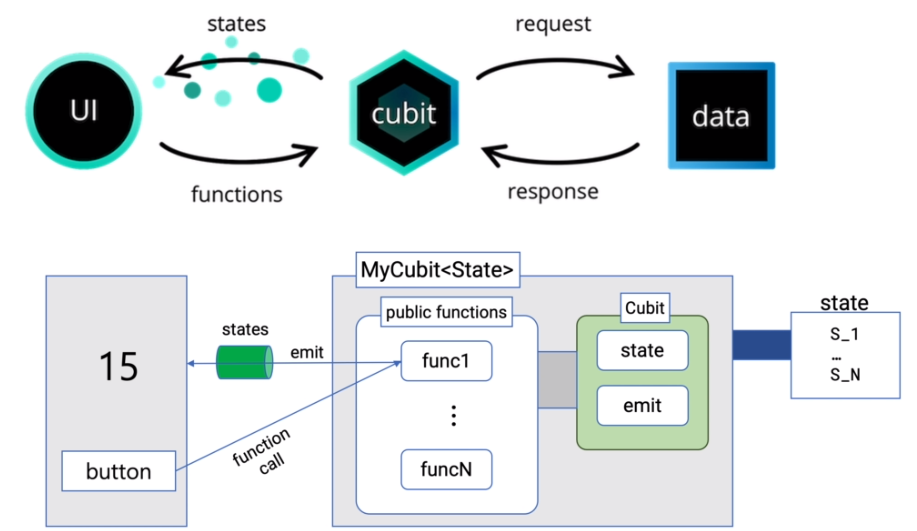
\includegraphics[width=9cm]{../libs/cubit-structure}
	\end{figure}
\end{frame}

%% ---------------------------------------------------------------------------

\begin{frame}{Cosa possiamo osservare}
	\begin{figure}[htpb]
		\centering
		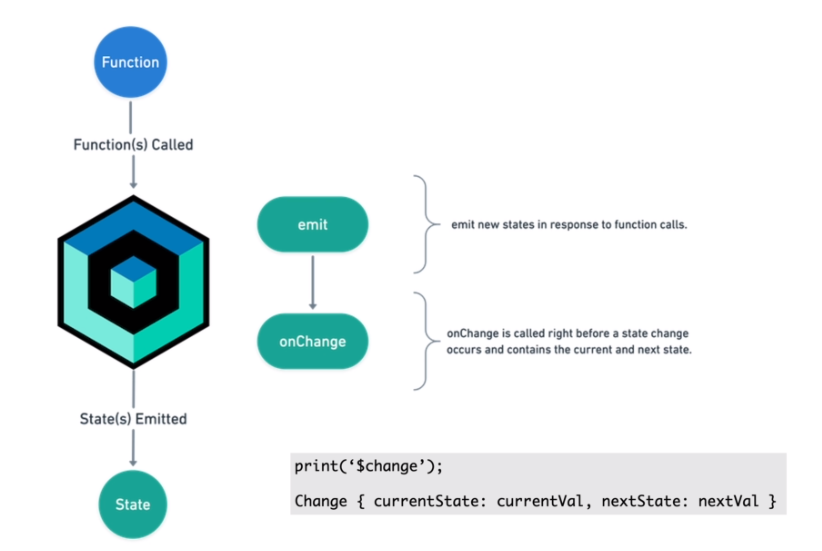
\includegraphics[width=9cm]{../libs/cubit-flow}
	\end{figure}
\end{frame}

%% ---------------------------------------------------------------------------

\begin{frame}{Cosa possiamo osservare - Confronto}
	\begin{figure}[htpb]
		\centering
		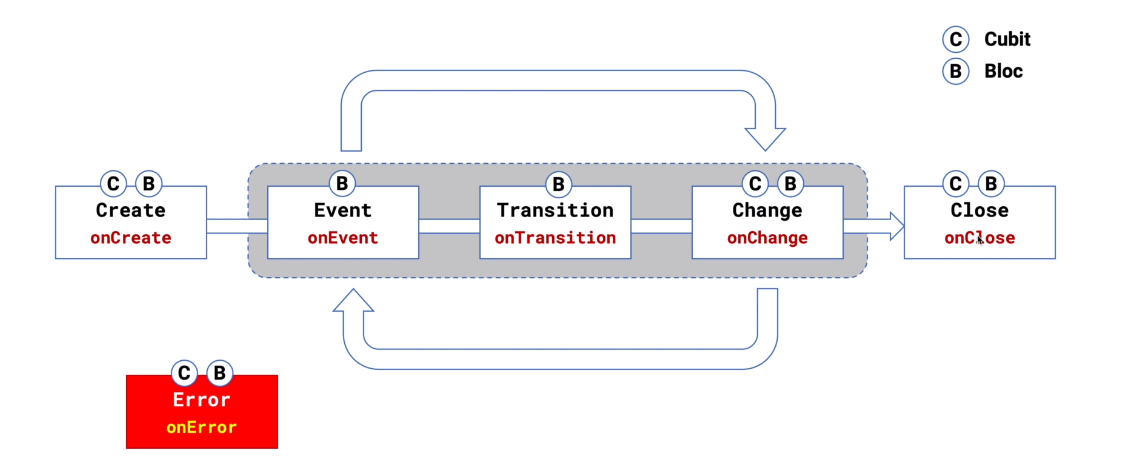
\includegraphics[width=9cm]{../libs/bloc-events}
	\end{figure}
\end{frame}

%% ---------------------------------------------------------------------------

\begin{frame}{Cubit vs BLoC}
	\begin{minipage}[0.2\textheight]{\textwidth}
		\begin{columns}[T]
			\begin{column}{0.4\textwidth}
				\begin{figure}[htpb]
					\centering
					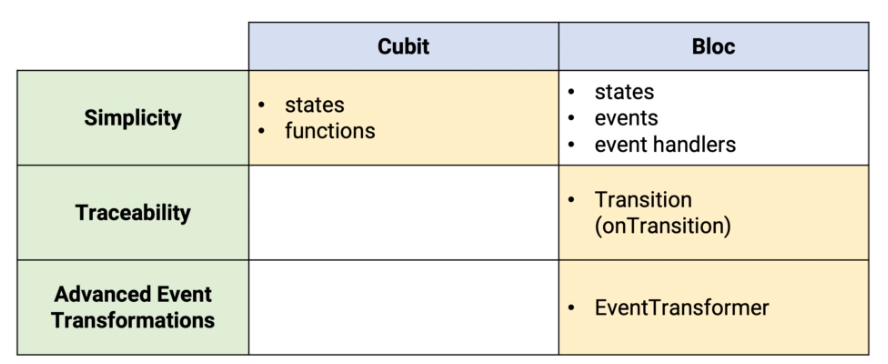
\includegraphics[scale=0.15]{../libs/cubit-bloc-diffs}
				\end{figure}
			\end{column}
			\begin{column}{0.6\textwidth}
				\begin{itemize}
					\item Una struttura ad eventi necessità di complessità aggiuntiva.
					\item Non sempre si ha bisogno di una gestione complessa.
					\item Si può sempre optare per soluzioni ibride, 	\emph{BLoC più Cubit}
				\end{itemize}
			\end{column}
		\end{columns}
	\end{minipage}
\end{frame}

%% ---------------------------------------------------------------------------

\section{BLoC - Come}
\begin{frame}{Rendere disponibile BLoC}
	\begin{minipage}[0.2\textheight]{\textwidth}
		\begin{columns}[T]
			\begin{column}{0.4\textwidth}
				\begin{figure}[htpb]
					\centering
					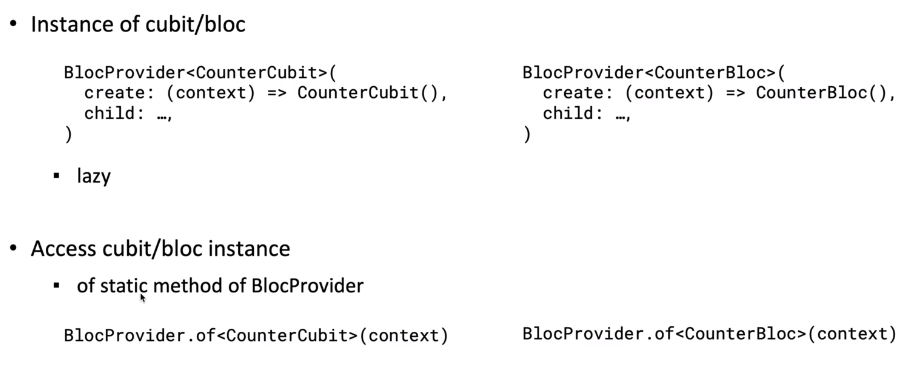
\includegraphics[scale=0.15]{../libs/bloc-provider}
				\end{figure}
			\end{column}
			\begin{column}{0.6\textwidth}
				\begin{itemize}
					\item Attraverso il provider rendiamo iniettabile nel sottoalbero il BLoC.
					\item Dal context recuperiamo il BLoC per l'utilizzo.
				\end{itemize}
			\end{column}
		\end{columns}
	\end{minipage}
\end{frame}

%% ---------------------------------------------------------------------------

\begin{frame}{BlocBuilder}
	\begin{figure}[htpb]
		\centering
		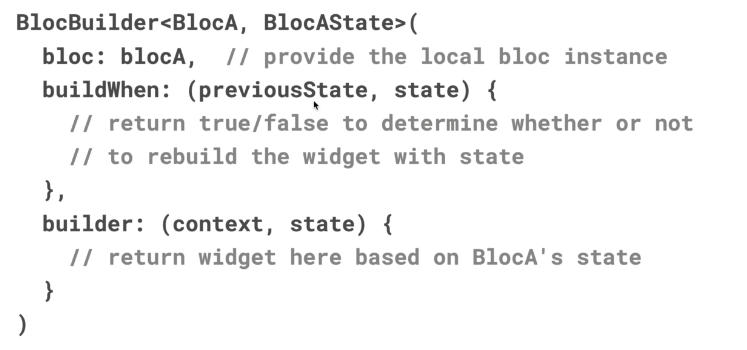
\includegraphics[width=9cm]{../libs/bloc-builder}
	\end{figure}
\end{frame}

%% ---------------------------------------------------------------------------

\begin{frame}{BlocListener}
	\begin{figure}[htpb]
		\centering
		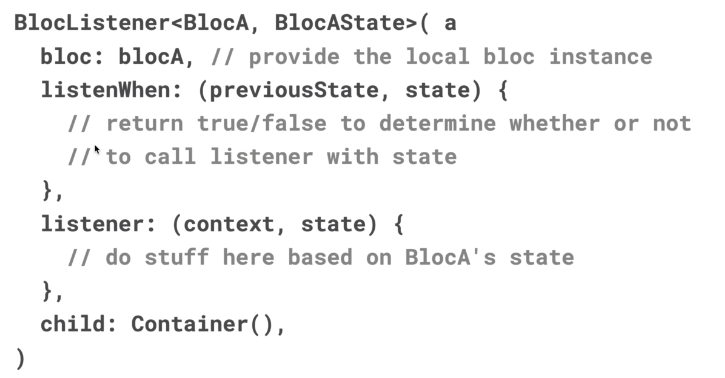
\includegraphics[width=9cm]{../libs/bloc-listener}
	\end{figure}
\end{frame}

%% ---------------------------------------------------------------------------

\begin{frame}{BlocConsumer}
	\begin{figure}[htpb]
		\centering
		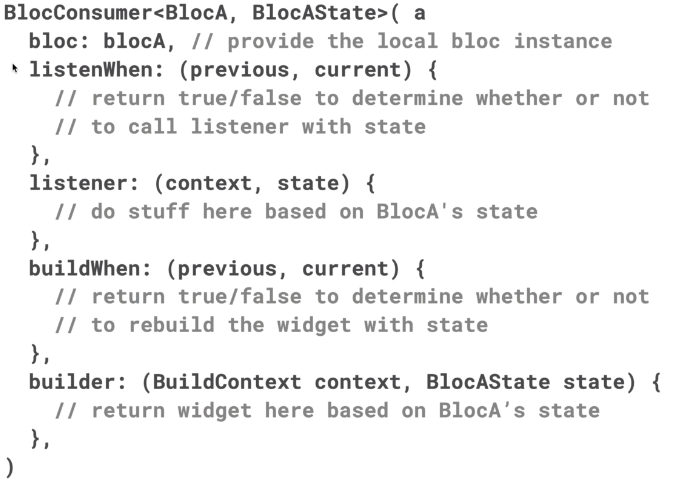
\includegraphics[width=9cm]{../libs/bloc-consumer}
	\end{figure}
\end{frame}

%% ---------------------------------------------------------------------------

\begin{frame}{Extension Methods}
	\begin{figure}[htpb]
		\centering
		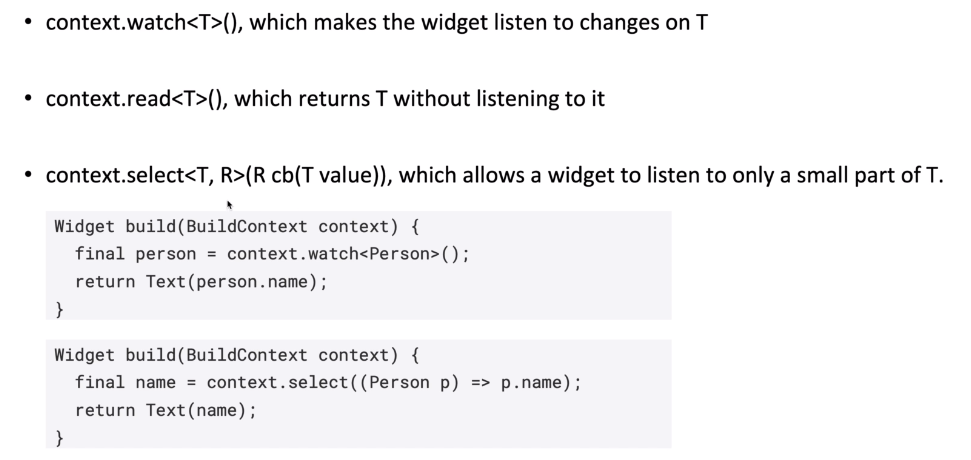
\includegraphics[width=9cm]{../libs/extension-methods}
	\end{figure}
\end{frame}

%% ---------------------------------------------------------------------------

\begin{frame}{Watch vs BlocBuilder}
	\begin{figure}[htpb]
		\centering
		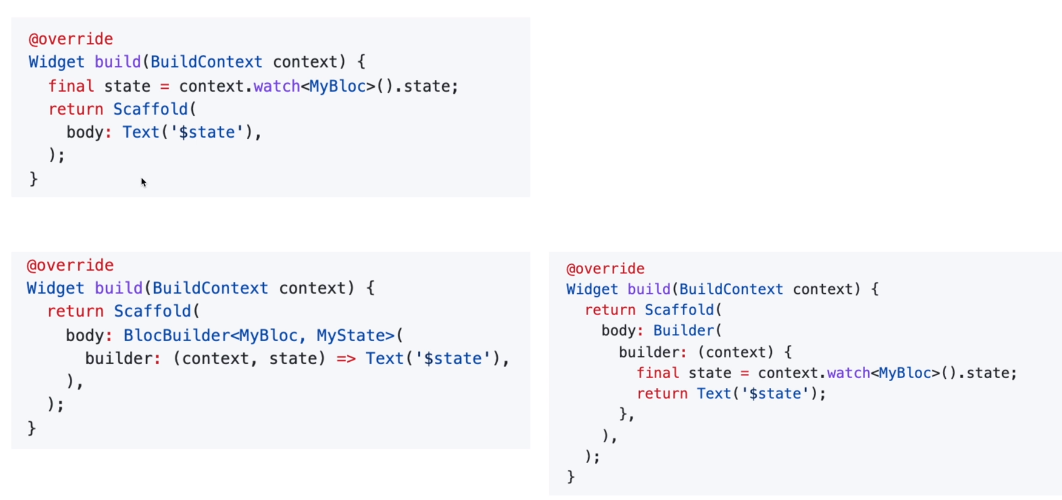
\includegraphics[width=9cm]{../libs/watch-vs-builder}
	\end{figure}
\end{frame}

%% ---------------------------------------------------------------------------

\begin{frame}{Cubits/BLoCs possono comunicare tra loro}
	\begin{figure}[htpb]
		\centering
		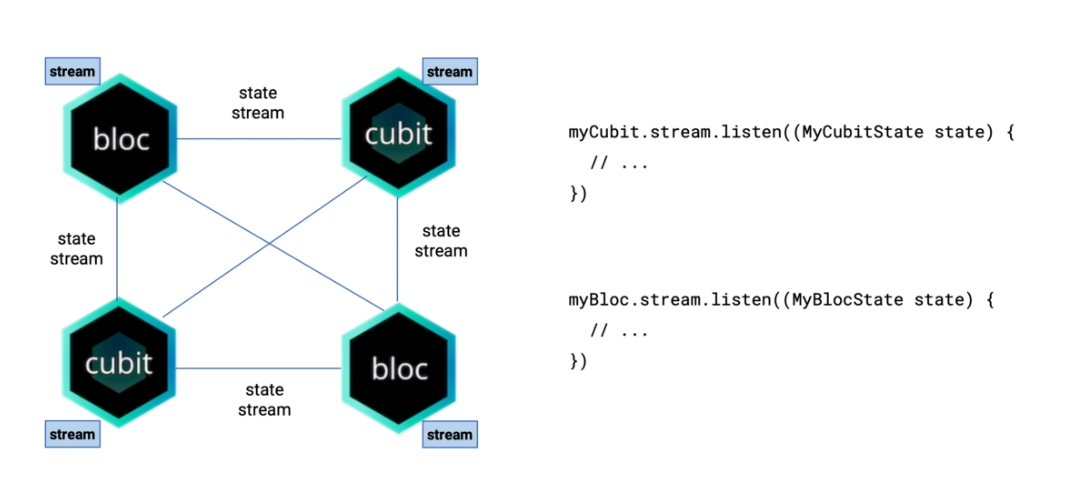
\includegraphics[width=9cm]{../libs/cubit-bloc-stream-communication}
	\end{figure}
\end{frame}

%% ---------------------------------------------------------------------------

\section{Esercitazione}
\begin{frame}{Migliorare la precedente esercitazione}
	\emph{Introdurre una gestione di memoria con Bloc/Cubit}
\end{frame}

%% ---------------------------------------------------------------------------

% Reference frames
%\begin{frame}[allowframebreaks]
%    \frametitle{Riferimenti}
%    \printbibliography
%\end{frame}

%% ---------------------------------------------------------------------------
% Final frame
\section{Fine}
\begin{frame}{}
	\huge\emph{Grazie per l'attenzione!}
	\newline
	\vfill
	\hfill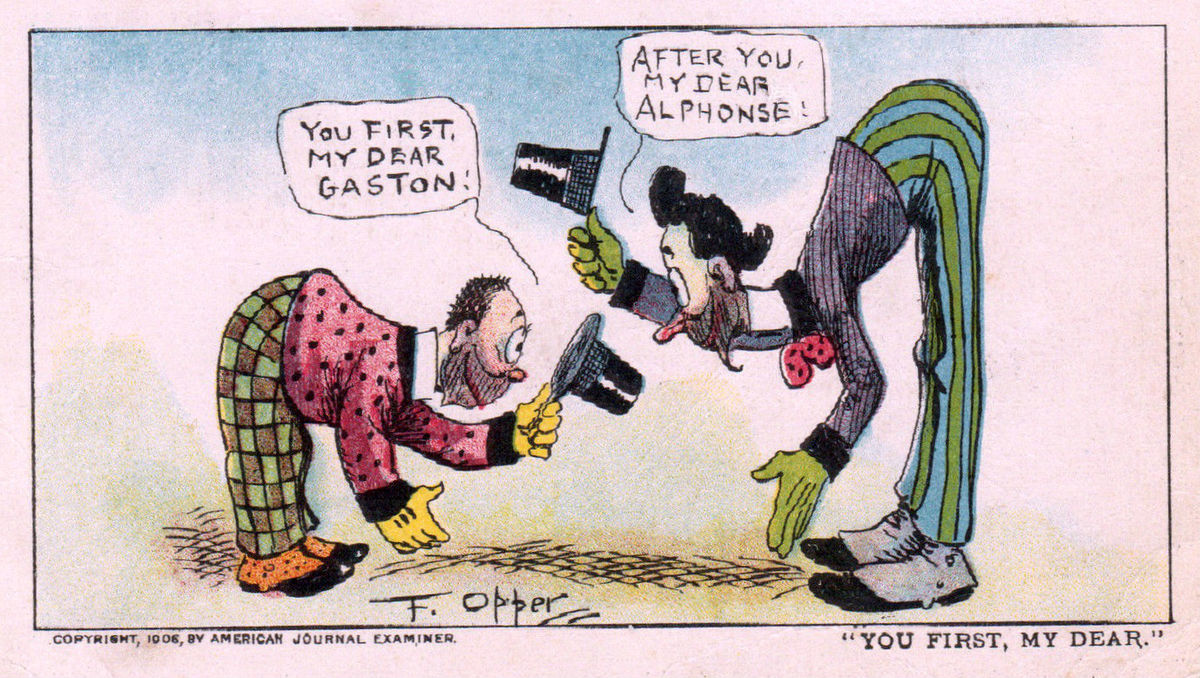
\includegraphics[width=6cm]{../libs/alphonse-gaston-regards}
\end{frame}

\end{document}